\documentclass{ximera}
\usetikzlibrary{patterns}
  \outcome{Understand the derivative of the accumulation function}
\begin{document}
\begin{problem}

  Suppose $f(a)$ is the area of the region---shown below---consisting of points $(x,y)$ where $0 \leq y \leq x$ and $0 \leq x \leq a$.
  \begin{image}
    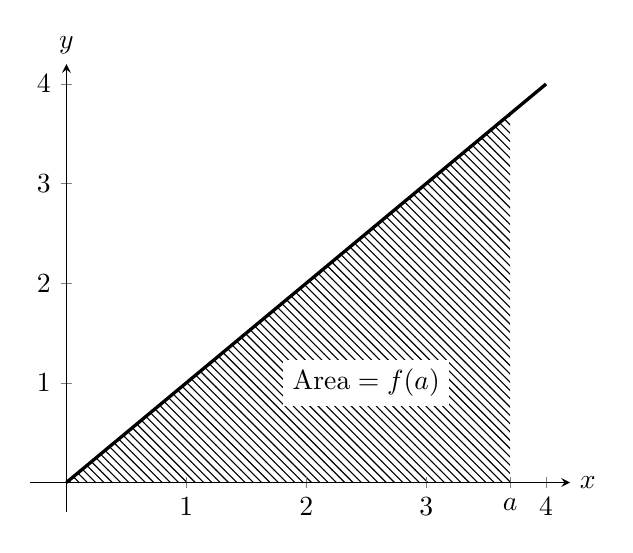
\begin{tikzpicture}
      \begin{axis}[
        clip=false,
        domain=0:4, 
        ytickmin=0,ytickmax=4,
        ytick={1,2,3,4},
        xtick={1,2,3,3.7,4},
        xticklabels={1,2,3,$a$,4},
        xtickmin=-10,xtickmax=10,
        ymin=-0.3, ymax=4.2,
        xmin=-0.3, xmax=4.2,
        xlabel=$x$, ylabel=$y$,
        axis lines=center,
        every axis y label/.style={at=(current axis.above origin),anchor=south},
        every axis x label/.style={at=(current axis.right of origin),anchor=west},
        axis on top,
        ]          
        \addplot [very thick,smooth] {x};
        \fill[pattern=north west lines] (axis cs:0,0) -- (axis cs:3.7,0) -- (axis cs:3.7,3.7) -- cycle;
        \node[fill=white,anchor=center] at (axis cs:2.5,1) {$\mbox{Area} = f(a)$};
      \end{axis}
    \end{tikzpicture}
    \end{image}
    What integer is closest to $\frac{f(4.01) - f(4)}{0.01}$?

  \begin{multipleChoice}
    \choice{0}
    \choice{1}
    \choice{2}
    \choice{3}
    \choice[correct]{4}
  \end{multipleChoice}
\end{problem}
\end{document}
